\documentclass{standalone}
\usepackage{tikz}
\usetikzlibrary{patterns, positioning}

\begin{document}
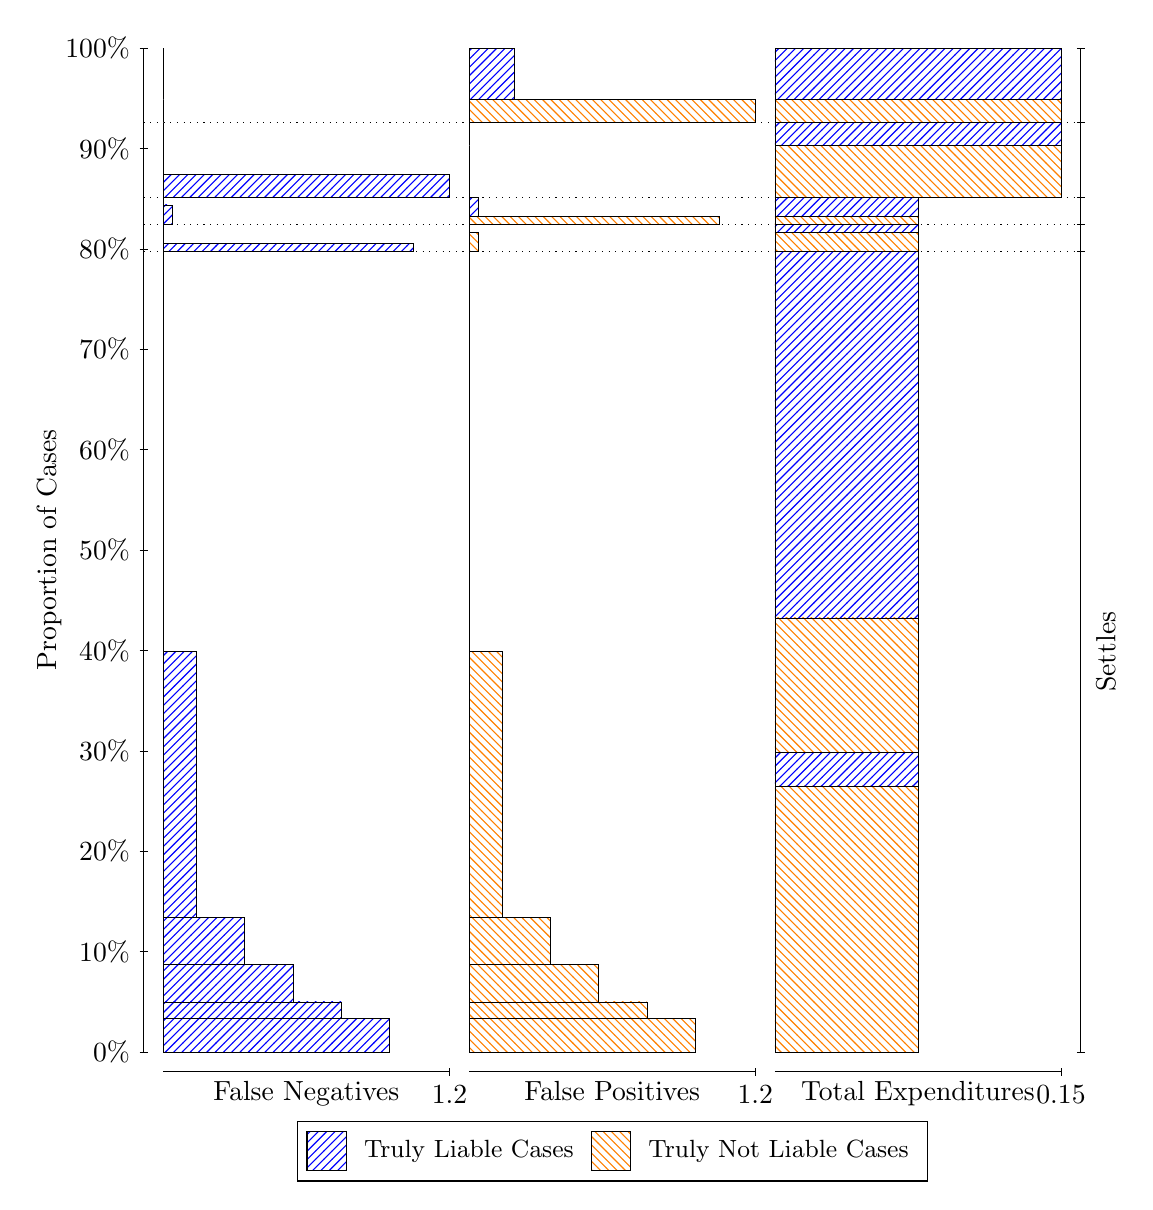
\begin{tikzpicture}
\draw[black, very thin] (1.5,1.75) -- (1.5,14.5);
\node[rotate=90, anchor=center] at (0.3, 8.125) {Proportion of Cases};
\draw[black, very thin] (1.45,1.75) -- (1.55,1.75);
\node[anchor=east] at (1.45, 1.75) {0\%};
\draw[black, very thin] (1.45,3.025) -- (1.55,3.025);
\node[anchor=east] at (1.45, 3.025) {10\%};
\draw[black, very thin] (1.45,4.3) -- (1.55,4.3);
\node[anchor=east] at (1.45, 4.3) {20\%};
\draw[black, very thin] (1.45,5.575) -- (1.55,5.575);
\node[anchor=east] at (1.45, 5.575) {30\%};
\draw[black, very thin] (1.45,6.85) -- (1.55,6.85);
\node[anchor=east] at (1.45, 6.85) {40\%};
\draw[black, very thin] (1.45,8.125) -- (1.55,8.125);
\node[anchor=east] at (1.45, 8.125) {50\%};
\draw[black, very thin] (1.45,9.4) -- (1.55,9.4);
\node[anchor=east] at (1.45, 9.4) {60\%};
\draw[black, very thin] (1.45,10.675) -- (1.55,10.675);
\node[anchor=east] at (1.45, 10.675) {70\%};
\draw[black, very thin] (1.45,11.95) -- (1.55,11.95);
\node[anchor=east] at (1.45, 11.95) {80\%};
\draw[black, very thin] (1.45,13.225) -- (1.55,13.225);
\node[anchor=east] at (1.45, 13.225) {90\%};
\draw[black, very thin] (1.45,14.5) -- (1.55,14.5);
\node[anchor=east] at (1.45, 14.5) {100\%};

\draw[black, very thin] (13.4,1.75) -- (13.4,14.5);
\draw[black, very thin] (13.35,1.75) -- (13.45,1.75);
\node[anchor=west] at (13.35, 1.75) {};
\draw[black, very thin] (13.35,11.916) -- (13.45,11.916);
\node[anchor=west] at (13.35, 11.916) {};
\draw[black, very thin] (13.35,12.261) -- (13.45,12.261);
\node[anchor=west] at (13.35, 12.261) {};
\draw[black, very thin] (13.35,12.606) -- (13.45,12.606);
\node[anchor=west] at (13.35, 12.606) {};
\draw[black, very thin] (13.35,13.553) -- (13.45,13.553);
\node[anchor=west] at (13.35, 13.553) {};
\draw[black, very thin] (13.35,14.5) -- (13.45,14.5);
\node[anchor=west] at (13.35, 14.5) {};

\draw[black, very thin, pattern color=blue, pattern=north east lines] (1.75,1.75) rectangle (4.6184,2.1788);
\draw[black, very thin, pattern color=blue, pattern=north east lines] (1.75,2.1788) rectangle (4.0065,2.3852);
\draw[black, very thin, pattern color=blue, pattern=north east lines] (1.75,2.3852) rectangle (3.3946,2.8666);
\draw[black, very thin, pattern color=blue, pattern=north east lines] (1.75,2.8666) rectangle (2.7826,3.4552);
\draw[black, very thin, pattern color=blue, pattern=north east lines] (1.75,3.4552) rectangle (2.1707,6.8332);
\draw[black, very thin, pattern color=orange, pattern=north west lines] (1.75,6.8332) rectangle (1.75,11.916);
\draw[black, very thin, pattern color=blue, pattern=north east lines] (1.75,11.916) rectangle (4.9244,12.015);
\draw[black, very thin, pattern color=orange, pattern=north west lines] (1.75,12.015) rectangle (1.75,12.261);
\draw[black, very thin, pattern color=blue, pattern=north east lines] (1.75,12.261) rectangle (1.8647,12.508);
\draw[black, very thin, pattern color=orange, pattern=north west lines] (1.75,12.508) rectangle (1.75,12.606);
\draw[black, very thin, pattern color=blue, pattern=north east lines] (1.75,12.606) rectangle (5.3833,12.9);
\draw[black, very thin, pattern color=orange, pattern=north west lines] (1.75,12.9) rectangle (1.75,13.553);
\draw[black, very thin, pattern color=orange, pattern=north west lines] (1.75,13.553) rectangle (1.75,13.847);
\draw[black, very thin, pattern color=blue, pattern=north east lines] (1.75,13.847) rectangle (1.75,14.5);
\draw[black, very thin, pattern color=orange, pattern=north west lines] (5.6333,1.75) rectangle (8.5018,2.1788);
\draw[black, very thin, pattern color=orange, pattern=north west lines] (5.6333,2.1788) rectangle (7.8898,2.3852);
\draw[black, very thin, pattern color=orange, pattern=north west lines] (5.6333,2.3852) rectangle (7.2779,2.8666);
\draw[black, very thin, pattern color=orange, pattern=north west lines] (5.6333,2.8666) rectangle (6.666,3.4552);
\draw[black, very thin, pattern color=orange, pattern=north west lines] (5.6333,3.4552) rectangle (6.054,6.8333);
\draw[black, very thin, pattern color=blue, pattern=north east lines] (5.6333,6.8333) rectangle (5.6333,11.916);
\draw[black, very thin, pattern color=orange, pattern=north west lines] (5.6333,11.916) rectangle (5.7481,12.163);
\draw[black, very thin, pattern color=blue, pattern=north east lines] (5.6333,12.163) rectangle (5.6333,12.261);
\draw[black, very thin, pattern color=orange, pattern=north west lines] (5.6333,12.261) rectangle (8.8077,12.36);
\draw[black, very thin, pattern color=blue, pattern=north east lines] (5.6333,12.36) rectangle (5.7481,12.606);
\draw[black, very thin, pattern color=orange, pattern=north west lines] (5.6333,12.606) rectangle (5.6333,13.259);
\draw[black, very thin, pattern color=blue, pattern=north east lines] (5.6333,13.259) rectangle (5.6333,13.553);
\draw[black, very thin, pattern color=orange, pattern=north west lines] (5.6333,13.553) rectangle (9.2667,13.847);
\draw[black, very thin, pattern color=blue, pattern=north east lines] (5.6333,13.847) rectangle (6.207,14.5);
\draw[black, very thin, pattern color=orange, pattern=north west lines] (9.5167,1.75) rectangle (11.333,5.1281);
\draw[black, very thin, pattern color=blue, pattern=north east lines] (9.5167,5.1281) rectangle (11.333,5.5569);
\draw[black, very thin, pattern color=orange, pattern=north west lines] (9.5167,5.5569) rectangle (11.333,7.2621);
\draw[black, very thin, pattern color=blue, pattern=north east lines] (9.5167,7.2621) rectangle (11.333,11.916);
\draw[black, very thin, pattern color=orange, pattern=north west lines] (9.5167,11.916) rectangle (11.333,12.163);
\draw[black, very thin, pattern color=blue, pattern=north east lines] (9.5167,12.163) rectangle (11.333,12.261);
\draw[black, very thin, pattern color=orange, pattern=north west lines] (9.5167,12.261) rectangle (11.333,12.36);
\draw[black, very thin, pattern color=blue, pattern=north east lines] (9.5167,12.36) rectangle (11.333,12.606);
\draw[black, very thin, pattern color=orange, pattern=north west lines] (9.5167,12.606) rectangle (13.15,13.259);
\draw[black, very thin, pattern color=blue, pattern=north east lines] (9.5167,13.259) rectangle (13.15,13.553);
\draw[black, very thin, pattern color=orange, pattern=north west lines] (9.5167,13.553) rectangle (13.15,13.847);
\draw[black, very thin, pattern color=blue, pattern=north east lines] (9.5167,13.847) rectangle (13.15,14.5);
\draw[black, dotted] (1.5,11.916) -- (13.4,11.916);
\draw[black, dotted] (1.5,12.261) -- (13.4,12.261);
\draw[black, dotted] (1.5,12.606) -- (13.4,12.606);
\draw[black, dotted] (1.5,13.553) -- (13.4,13.553);
\draw[black, very thin] (1.75,1.5) -- (5.3833,1.5);
\node[anchor=north] at (3.5667, 1.5) {False Negatives};
\draw[black, very thin] (5.3833,1.45) -- (5.3833,1.55);
\node[anchor=north] at (5.3833, 1.45) {1.2};

\draw[black, very thin] (5.6333,1.5) -- (9.2667,1.5);
\node[anchor=north] at (7.45, 1.5) {False Positives};
\draw[black, very thin] (9.2667,1.45) -- (9.2667,1.55);
\node[anchor=north] at (9.2667, 1.45) {1.2};

\draw[black, very thin] (9.5167,1.5) -- (13.15,1.5);
\node[anchor=north] at (11.333, 1.5) {Total Expenditures};
\draw[black, very thin] (13.15,1.45) -- (13.15,1.55);
\node[anchor=north] at (13.15, 1.45) {0.15};

\node[black, centered, rotate=90] at (13.72, 6.8332) {Settles};





\draw (7.449999999999999,1.5) node[draw=none] (baseCoordinate) {};
\begin{scope}[align=center]
        \matrix[scale=0.5, draw=black, below=0.5cm of baseCoordinate, nodes={draw}, column sep=0.1cm]{
            \node[rectangle, draw, minimum width=0.5cm, minimum height=0.5cm, pattern=north east lines, pattern color=blue] {}; &
            \node[draw=none, font=\small] (B) {Truly Liable Cases}; &
            \node[rectangle, draw, minimum width=0.5cm, minimum height=0.5cm, pattern=north west lines, pattern color=orange] {}; &
            \node[draw=none, font=\small] (B) {Truly Not Liable Cases}; \\
            };
\end{scope}

\end{tikzpicture}
\end{document}